%%%%%%%%%%%%%%%%%%%%%%%%%%%%%%%%%%%%%%%%%%%%%%%%%%%%%%%%%%%%%%%%%%
%%%%%%%% ICML 2013 EXAMPLE LATEX SUBMISSION FILE %%%%%%%%%%%%%%%%%
%%%%%%%%%%%%%%%%%%%%%%%%%%%%%%%%%%%%%%%%%%%%%%%%%%%%%%%%%%%%%%%%%%

% Use the following line _only_ if you're still using LaTeX 2.09.
%\documentstyle[icml2013,epsf,natbib]{article}
% If you rely on Latex2e packages, like most moden people use this:
\documentclass{article}

% For figures
\usepackage{graphicx} % more modern
%\usepackage{epsfig} % less modern
\usepackage{subfigure} 

% For citations
\usepackage{natbib}

% For algorithms
\usepackage{algorithm}
\usepackage{algorithmic}

% As of 2011, we use the hyperref package to produce hyperlinks in the
% resulting PDF.  If this breaks your system, please commend out the
% following usepackage line and replace \usepackage{icml2013} with
% \usepackage[nohyperref]{icml2013} above.
\usepackage{hyperref}

% Packages hyperref and algorithmic misbehave sometimes.  We can fix
% this with the following command.
\newcommand{\theHalgorithm}{\arabic{algorithm}}

% Employ the following version of the ``usepackage'' statement for
% submitting the draft version of the paper for review.  This will set
% the note in the first column to ``Under review.  Do not distribute.''
\usepackage{icml2013} 
% Employ this version of the ``usepackage'' statement after the paper has
% been accepted, when creating the final version.  This will set the
% note in the first column to ``Proceedings of the...''
% \usepackage[accepted]{icml2013}


% The \icmltitle you define below is probably too long as a header.
% Therefore, a short form for the running title is supplied here:
\icmltitlerunning{Submission and Formatting Instructions for ICML 2013}

\begin{document} 

\twocolumn[
\icmltitle{Using K-Nearest Neighbors on the MNIST Dataset}

% It is OKAY to include author information, even for blind
% submissions: the style file will automatically remove it for you
% unless you've provided the [accepted] option to the icml2013
% package.
\icmlauthor{Carl Cortright}{carl.cortright@colorado.edu}

% You may provide any keywords that you 
% find helpful for describing your paper; these are used to populate 
% the "keywords" metadata in the PDF but will not be shown in the document
\icmlkeywords{boring formatting information, machine learning, ICML}

\vskip 0.3in
]

\section{Introduction}

In this assignment, I use a K-Nearest-Neighbors (KNN) model, implemented using scikit-learn and numpy, to classify the MNIST handwriting dataset. I then show how the role of the number of datapoints as well as K contribute to accuracy. Afterwards I analyze which numbers get confused with eachother most easily. 

\section{Analysis}

After completing the model, I ran a series of trials comparing the number of training examples with the accuracy while holding k constant. Before running the test I hypothesized that as we gave the model more training examples we would have higher accuracy. By graphing the results it is clear that the accuracy is asymptotically approaching somewhere around 95-96 percent.

\begin{figure}[!ht]

  \caption{Graph of KNN Accuracy vs. Training example limit.}
  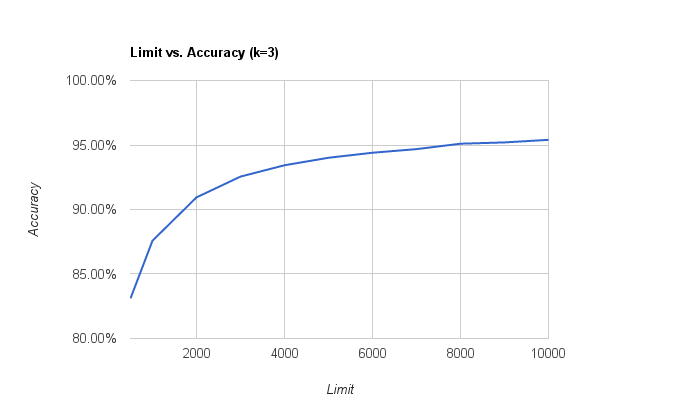
\includegraphics[width=\columnwidth]{limit.png}

\end{figure}

Next I plotted accuracy vs k. I decided to keep the limit set to 500 because at 500 the change in accuracy would be easier to see with change in k. The results were interesting; as k grew the accuracy sinusoidally approached somewhere around 79 percent.

\begin{figure}[!ht]

  \caption{Graph of KNN Accuracy vs. k.}
  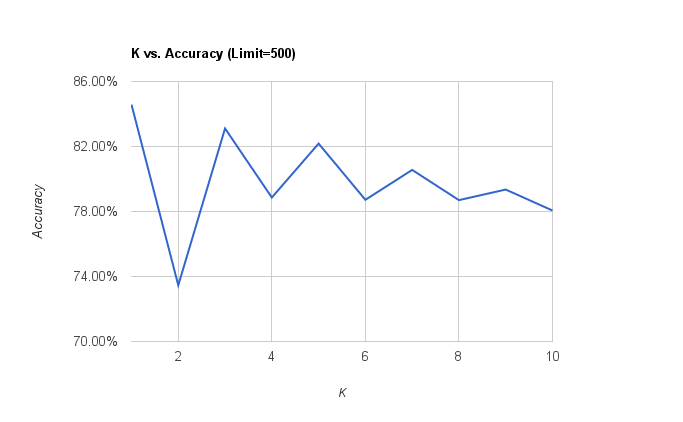
\includegraphics[width=\columnwidth]{k.png}

\end{figure}

Another interesting metric to consider with the MNIST dataset is what numbers get confused with other numbers. It is easy to analyze using the confusion matrix printed at the end of the program. By analyzing this matrix, you can see that the numbers 5 and 8 get confused with other numbers most often. The number 5 mostly gets confused with the numbers 3 and 6 whereas 8 gets confused with 3 and 5. Another outlier is how the number four gets confused with 9, an occurance that happend 19 times in our test. All of these confusions make sense due to the numbers that are being confused looking somewhat similar. It would be weird if 1 got confused with 5 because they look nothing alike. The vectors representing 8 and 3 on the other hand must look very similar due to their curved nature.

\begin{figure}[!ht]

  \caption{Confusion Matrix with final accuracy of 97 percent}
  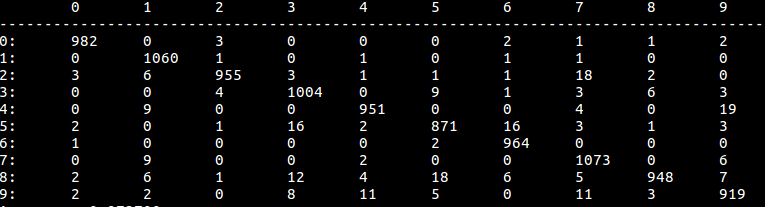
\includegraphics[width=\columnwidth]{ConfusionMatrix.png}

\end{figure}


\section{Conclusion}

In this assignment I analyzed how accuracy was effected by comparing it to both the k value and the limit of training examples. I then analyzed what numbers were getting confused the most. The final accuracy was achieved was slightly above 97 percent which makes it acceptable in the research context but still less accurate than methods like deep learning. 

\end{document} 


% This document was modified from the file originally made available by
% Pat Langley and Andrea Danyluk for ICML-2K. This version was
% created by Lise Getoor and Tobias Scheffer, it was slightly modified  
% from the 2010 version by Thorsten Joachims & Johannes Fuernkranz, 
% slightly modified from the 2009 version by Kiri Wagstaff and 
% Sam Roweis's 2008 version, which is slightly modified from 
% Prasad Tadepalli's 2007 version which is a lightly 
% changed version of the previous year's version by Andrew Moore, 
% which was in turn edited from those of Kristian Kersting and 
% Codrina Lauth. Alex Smola contributed to the algorithmic style files.  
